%----------------------------------------------------------------------------------------
%	PACKAGES AND THEMES
%----------------------------------------------------------------------------------------

\documentclass{beamer}

\mode<presentation> {
\usetheme{Madrid}
\setbeamertemplate{navigation symbols}{}
}

\usepackage{graphicx} % Allows including images
\usepackage{booktabs} % Allows the use of \toprule, \midrule and \bottomrule in tables
\usepackage[english]{babel}
\usepackage[utf8]{inputenc}
\usepackage[normalem]{ulem}
\usepackage{multicol}
\usepackage[backend=bibtex, sorting=none, maxbibnames=99]{biblatex}

\usepackage{hyperref}
\usepackage{mathpartir}
\usepackage{xspace}
\usepackage{pgfplots}
\pgfplotsset{width=7cm,compat=1.8}
\usepackage{pgfplotstable}

\newcommand{\lang}{\textsc{Effy}\xspace}
\newcommand{\eff}{\textsc{Eff}\xspace}
\newcommand{\ocaml}{\textsc{OCaml}\xspace}

% Meta-syntax
\newcommand{\bnfis}{\mathrel{\;{:}{:}\!=}\;}
\newcommand{\bnfor}{\mathrel{\;|\;}}
\newcommand{\defeq}{\mathrel{\;\stackrel{\text{def}}{=}\;}}
\newcommand{\set}[1]{\{ #1 \}}

% General syntactic constructs
\newcommand{\kord}[1]{\mathtt{#1}}
\newcommand{\kop}[1]{\;\mathtt{#1}\;}
\newcommand{\kpre}[1]{\mathtt{#1}\;}
\newcommand{\kpost}[1]{\;\mathtt{#1}}

% Types
\newcommand{\type}[1]{\mathtt{#1}}
\newcommand{\boolty}{\type{bool}}
\newcommand{\intty}{\type{int}}
\newcommand{\hto}{\Rightarrow}
\newcommand{\C}{\underline{C}}
\newcommand{\D}{\underline{D}}
\newcommand{\dirt}{\Delta}
\newcommand{\sig}{\Sigma}

% Expressions and computations
\newcommand{\call}[3]{{{#1}\,{#2}\,{#3}}}
\newcommand{\case}{\mathop{\text{\texttt{|}}}}
\newcommand{\cont}[2]{(#1.\,#2)}
\newcommand{\const}{\kord{k}}
\newcommand{\fls}{\kord{false}}
\newcommand{\fun}[1]{\kpre{fun} #1 \mapsto}
\newcommand{\handler}[1]{\{ #1 \}}
\newcommand{\conditional}[3]{\kpre{if} #1 \kop{then} #2 \kop{else} #3}
\newcommand{\letin}[1]{\kpre{let} #1 \kop{in}}
\newcommand{\doin}[1]{\kpre{do} #1 \kop{ ; }}
\newcommand{\letrecin}[1]{\kpre{let} \kpre{rec} #1 \kop{in}}
\newcommand{\op}{\kord{Op}}
\newcommand{\ops}{\mathcal{O}}
\newcommand{\ocs}{\mathit{ocs}}
\newcommand{\ocsnil}{\kord{nil}}
\newcommand{\tru}{\kord{true}}
\newcommand{\ret}{\kpre{return}}
\newcommand{\withhandle}[2]{\kpre{handle} #2 \kop{with} #1}
\newcommand{\pure}[1]{\kord{pure } #1  }
\newcommand{\longcases}{\call{\op_1}{x}{k} \mapsto c_{\op_1}, \ldots, \call{\op_n}{x}{k} \mapsto c_{\op_n}}
\newcommand{\shortcases}{[\call{\op}{x}{k} \mapsto c_\op]_{\op \in \ops}}
\newcommand{\longhand}[1][\ret x \mapsto c_r]{\handler{#1, \longcases}}
\newcommand{\shorthand}[1][\ret x \mapsto c_r]{\handler{#1, \shortcases}}

% Type-checking
\newcommand{\ctx}{\Gamma}
\newcommand{\ent}{\vdash}
\newcommand{\T}{\mathrel{:}}
\newcommand{\E}{\mathrel{!}}
\newcommand{\covers}{\mathrel{/}}
\renewcommand{\le}{\leqslant}

% Operational semantics
\newcommand{\eval}{\Downarrow}
\newcommand{\hs}{\mathcal{H}}
\newcommand{\nil}{\emptyset}
\newcommand{\cons}{\mathbin{::}}
\newcommand{\hseval}[1][\hs]{\Downarrow_{#1}}
\newcommand{\getval}[1]{{#1}_{\kord{val}}}
\newcommand{\getop}[1]{{#1}_{\kord{op}}}

%functions

\newcommand{\inlinable}[3]{\textit{inlinable(}#1, #2 ,#3 \textit{)}}


\newcommand{\queens}[1]{\textit{#1-Queens}\xspace}
\newcommand{\loops}{\textit{Loop}}

\bibliography{presentation}
\def\bibfont{\footnotesize}

\usepackage{listings}
\lstset{
language=caml,
basicstyle=\small\ttfamily,
columns=flexible,
breaklines=true,
keywordstyle=\color{blue}\ttfamily,
stringstyle=\color{red}\ttfamily,
commentstyle=\color{green}\ttfamily
}

%----------------------------------------------------------------------------------------
%	TITLE PAGE
%----------------------------------------------------------------------------------------

\title[Honoursprogramme: Research track]{
Honoursprogramme: Research track, option A (9 ECTS) \\
\large Efficient Compilation of Algebraic Effects and Handlers in Eff} % The short title appears at the bottom of every slide, the full title is only on the title page

\author[Axel Faes]{
Axel Faes
} 

\institute[KUL] % Your institution as it will appear on the bottom of every slide, may be shorthand to save space
{
prof. dr. ir. Tom Schrijvers\\
Amr Hany Shehata Saleh\\\mbox{}\\
Master in de ingenieurswetenschappen: computerwetenschappen (fase 1) \\
Specialisatie: Artificiel Intelligence \\
\medskip
KULeuven % Your institution for the title page
}
\date{September 2016 - March 2017} % Date, can be changed to a custom date

\begin{document}

\begin{frame}
\titlepage % Print the title page as the first slide
\end{frame}

\begin{frame}{\contentsname}
\frametitle{Table of Contents} % Table of contents slide, comment this block out to remove it
%\begin{multicols}{2}
\tableofcontents
%\end{multicols}
\end{frame}

%----------------------------------------------------------------------------------------
%	PRESENTATION SLIDES
%----------------------------------------------------------------------------------------

\section{Description}
\subsection{Introduction}
\subsection{Literature study}
\subsection{Optimizations}
\subsection{Benchmarks}
\subsection{Results}

\section{Reflection}
\subsection{General}
\subsection{Link to degree}
\subsection{Oral communication}
\subsection{Written communication}
\subsection{Theoretical and mathematical foundations of computer science}
\subsection{Asking for help}
\subsection{Time management}
\subsection{Creating a hypothesis}

\section{Conclusion}
\section{References}

%------------------------------------------------

\begin{frame}[fragile]
\frametitle{Description}
\framesubtitle{Introduction}

\begin{columns}[T] % align columns
\begin{column}{.48\textwidth}

	\textbf{Overview}
	\begin{itemize}
	\item Part of C1 project \cite{project}
	\item Eff programming language \cite{eff}
	\item Type-\&-effect system
	\item Compile to OCaml
	\item No optimizations $=>$ slow execution \cite{KCeff}
	\end{itemize}

	\textbf{Steps}
	\begin{itemize}
	\item Literature study
	\item Optimizations
	\item Benchmarks
	\item \sout{Formal proof}
	\end{itemize}
	
\end{column}%
\hfill%
\begin{column}{.48\textwidth}

	\begin{block}{Eff: N-queens sample code}
	\begin{lstlisting}
effect Decide : unit -> bool
effect Fail : unit -> empty

let choose_all = handler
  | val x -> [x]
  | #Decide _ k -> k true @ k false
  | #Fail _ _ -> []

let queens_all nb_of_queens =
  with choose_all handle queens nb_of_queens
	\end{lstlisting}
	\end{block}

\end{column}%
\end{columns}

\end{frame}

%------------------------------------------------

\begin{frame}[fragile]
\frametitle{Description}
\textbf{Literature study}
\begin{itemize}
\item Papers about algebraic effect handlers \cite{monads} \cite{effectsystem} \cite{inferring} \cite{handling}
\item Papers about Eff \cite{introduction}  \cite{programming}
\item Getting familiar with compiler
\end{itemize}

\textbf{Optimizations}
\begin{itemize}
\item with h handle (c) [c is pure for h] $=>$ c
\item with h handle (c1 $>>$ c2) [c1 is pure for h] $=>$ c1 $>>$ (with h handle (c2))
\item with h handle (c1 $>>$ c2) [c2 is pure for h] $=>$ with h' handle (c1) {[h' = c2 $>>$ h.value\_clause]}
\item with h handle (c1 $>>$ c2) $=>$ with h' handle (c1) {[h' = with h handle c2]}
\item with h handle (let rec defs = ... in c) $=>$ let rec defs = ... in (with h handle c)
\end{itemize}
\end{frame}

%------------------------------------------------

%\begin{frame}[fragile]
%\frametitle{Description}
%\framesubtitle{Optimizations}
%
%\begin{figure}[h!]
%\begin{center}
%\framebox{
%\begin{minipage}{0.95\columnwidth}
%\textbf{Handler Reduction}
%\begin{mathpar}
%  \inferrule[With-Pure]{
%     h = \shorthand \\
%     \Gamma \vdash c : A \E \dirt \\
%     \dirt \cap \ops = \emptyset
%  }{
%    \withhandle{h}{c} \leadsto \doin{x \leftarrow c} c_r
%  }
%
%  \inferrule[With-Do]{
%    h = \shorthand \\
%    h' = \shorthand[\ret y \mapsto (\withhandle{h}{c_2})]
%  }
%    {
%    \withhandle{h}{(\doin{y \leftarrow c_1} c_2)} \leadsto
%    \withhandle{h'}{c_1}
%  }
%\end{mathpar}
%\end{minipage}
%}
%\end{center}
%\caption{Term Rewriting Rules \cite{own}}\label{fig:rewriterules}
%\end{figure}
%\end{frame}

%------------------------------------------------

%\begin{frame}[fragile]
%\frametitle{Description}
%\framesubtitle{Optimizations}
%
%\begin{figure}[h!]
%\begin{center}
%\framebox{
%\begin{minipage}{0.95\columnwidth}
%\textbf{Handler Reduction}
%\begin{mathpar}
%  \inferrule[With-LetRec]{
%  }{
%    \withhandle{v}{(\letrecin{f \, x = c_1} c_2)} \leadsto
%    \letrecin{f \, x = c_1} \\(\withhandle{v}{c_2}) 
%  }
%\end{mathpar}
%\end{minipage}
%}
%\end{center}
%\caption{Term Rewriting Rules \cite{own}}\label{fig:rewriterules}
%\end{figure}
%\end{frame}

%------------------------------------------------

\begin{frame}[fragile]
\frametitle{Description}
\framesubtitle{Benchmarks}
\begin{columns}[T] % align columns
\begin{column}{.48\textwidth}
	
	\textbf{Eff benchmarks}
	\begin{itemize}
	\item Loops
	\item N-queens
	\item Interpreter \cite{interpreter}
	\item Parser \cite{scope}
	\end{itemize}	
	
\end{column}%
\hfill%
\begin{column}{.48\textwidth}

	\textbf{Other systems}
	\begin{itemize}
	\item Handlers in Action \cite{handlersinaction} \cite{delimccweb}
	\item Eff directly in OCaml \cite{directly} \cite{delimccweb}
	\item Multicore OCaml \cite{multicore}
	\item \sout{Links} \cite{linkslang} \cite{links} \cite{Hillerstrom:2016:LER:2976022.2976033}
	\end{itemize} \mbox{}\\
	
	\textbf{Method of testing}
	\begin{itemize}
	\item Bytecode
	\item Binary
	\end{itemize}

\end{column}%
\end{columns}
\end{frame}

%------------------------------------------------

\begin{frame}[fragile, allowframebreaks]
\frametitle{Description}
\framesubtitle{Results}

\begin{figure}[h!]
\centering
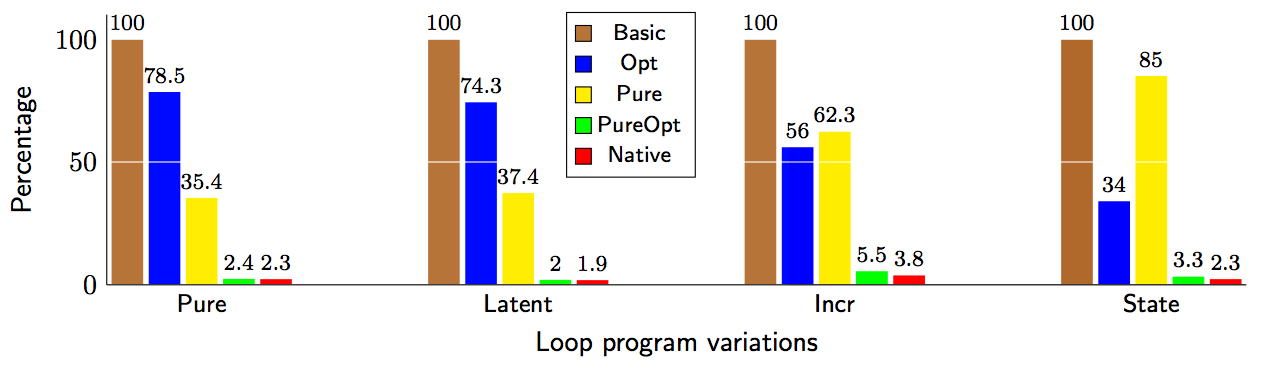
\includegraphics[width=\textwidth]{loop}
\caption{Relative run-times of Loops example  \cite{own}}
\label{fig:loops}
\end{figure}

\begin{figure}[h!]
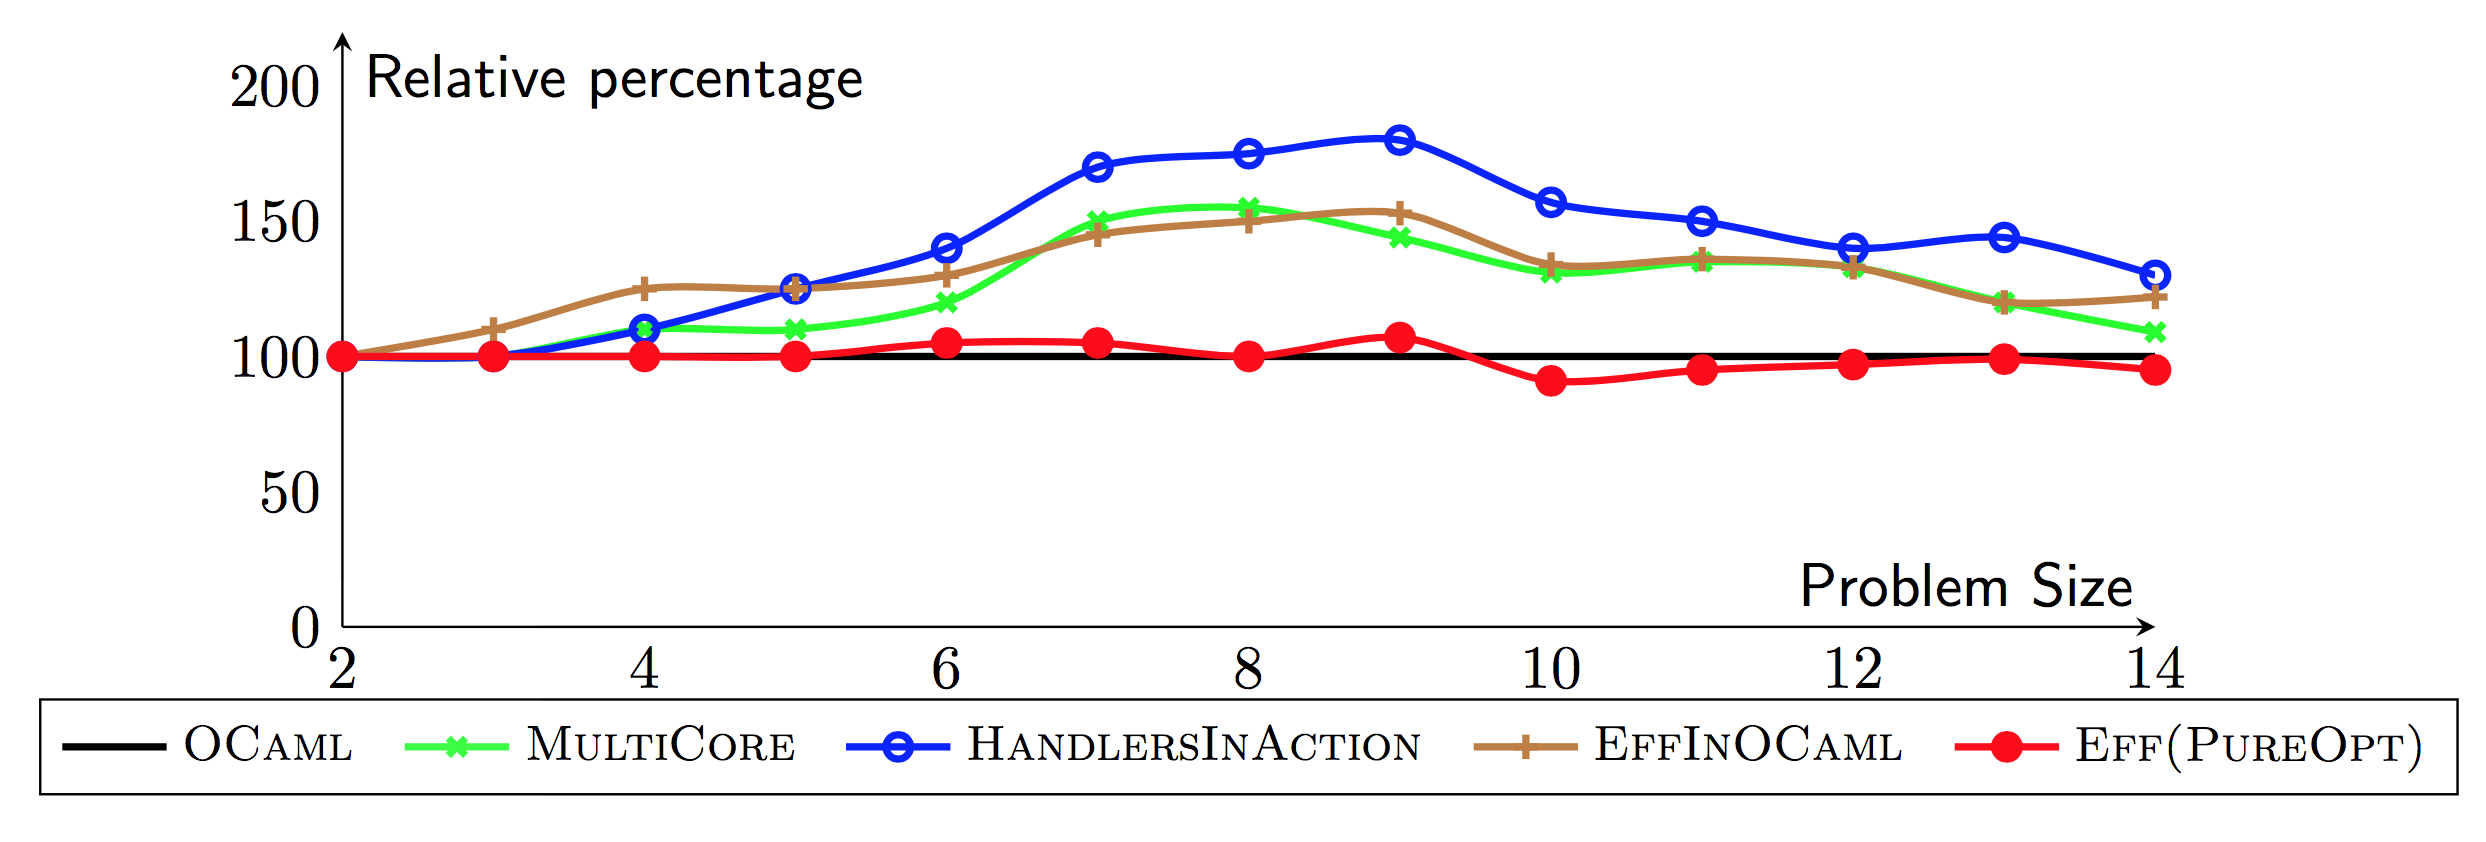
\includegraphics[width=\textwidth]{allqueens}
\caption{Results of running N-Queens for all solutions on multiple systems  \cite{own}}
\label{fig:systemsall}
\end{figure}

%\begin{figure}[h!]
%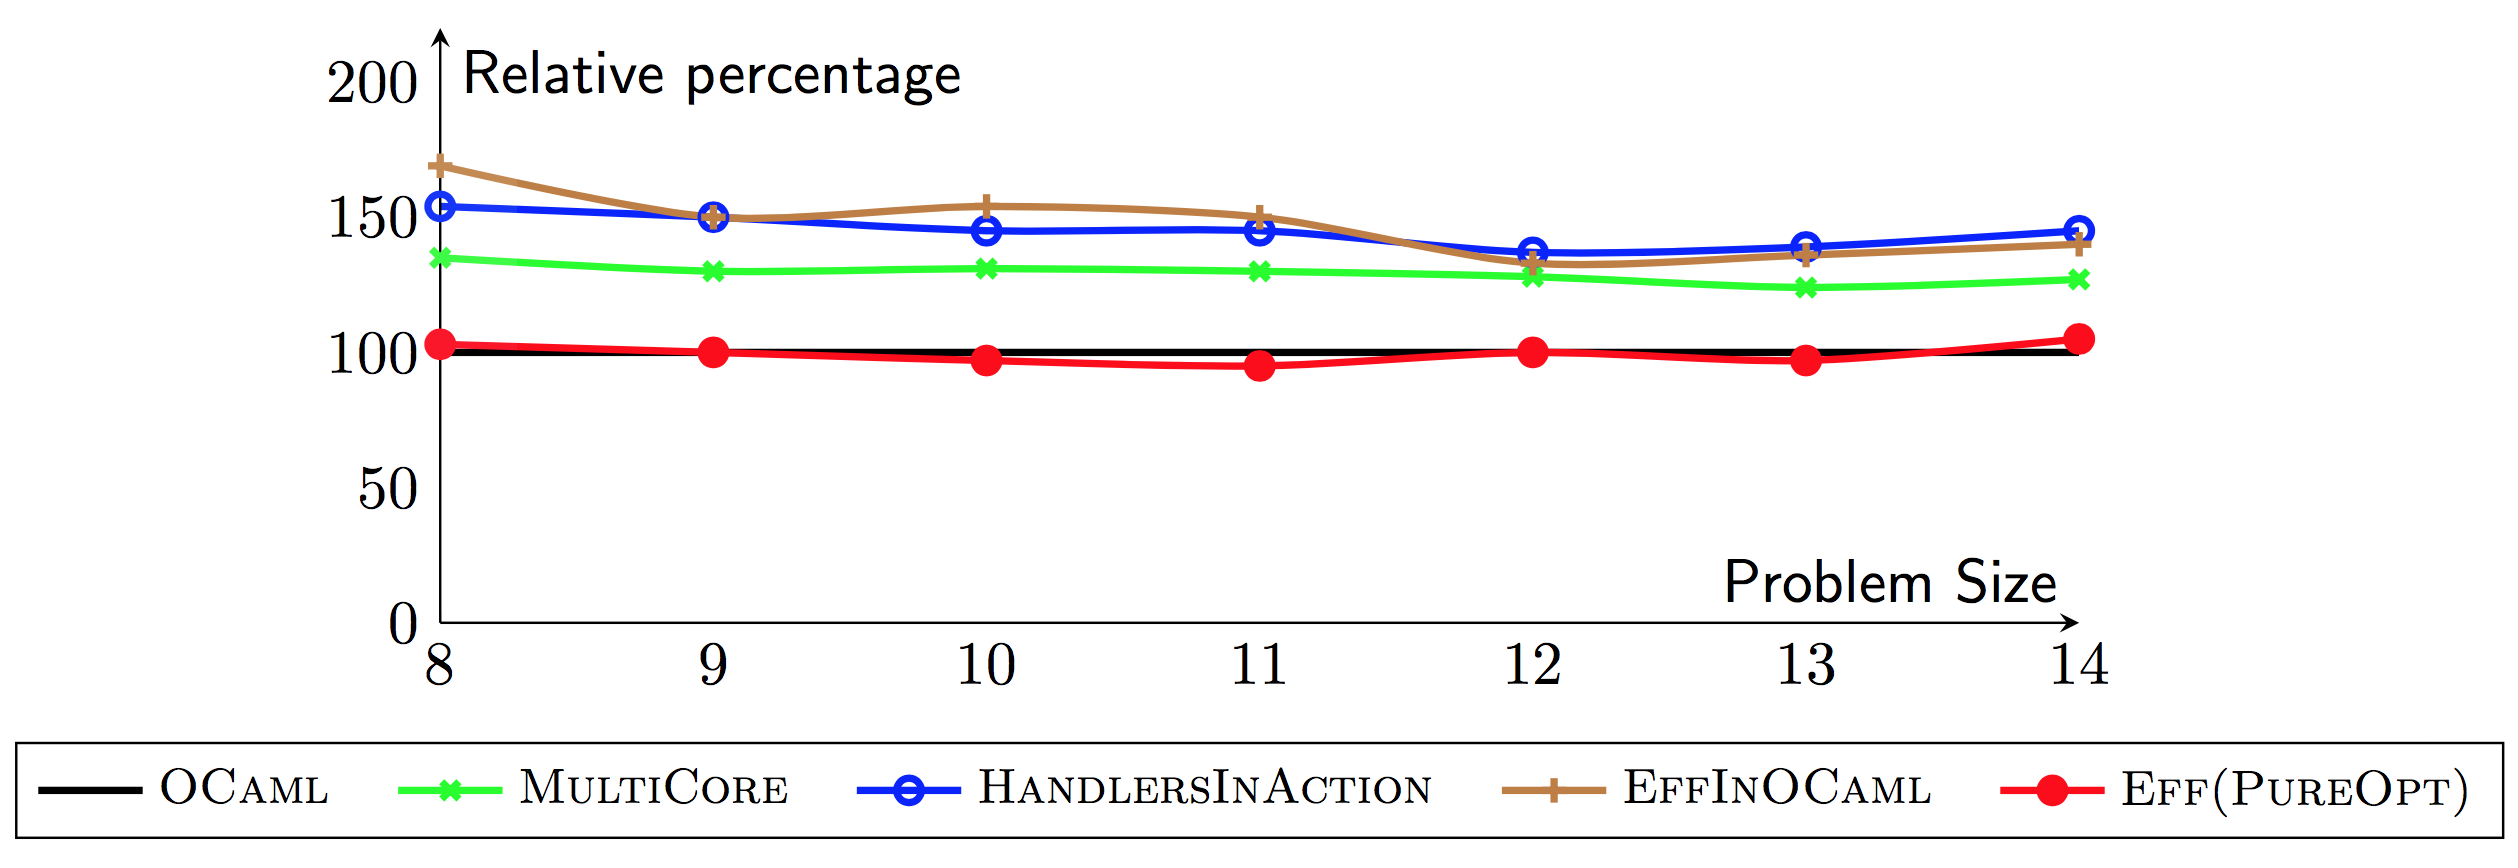
\includegraphics[width=\textwidth]{onequeens}
%\caption{Results of running N-Queens for one solution on multiple systems  \cite{own}}
%\label{fig:systemsone}
%\end{figure}

\end{frame}

%------------------------------------------------

\begin{frame}[fragile]
\frametitle{Reflection}
\textbf{General reflection}
\begin{itemize}
\item Opportunity to perform research
\item Challenging
\item Done is one semester instead of throughout the year
\item Effect of 70 ECTS + honours $=>$ huge workload
\item Helped decide topic masterthesis
\item Helped decide second honoursproject
\end{itemize}

\textbf{Relation between honoursprogramme and degree}
\begin{itemize}
\item Was familiar with functional programming
\item Was familiar with compilers
\item Formal Systems and their Applications (H04H8BE)
\item Indirect synergy with other courses
\end{itemize}
\end{frame}

%------------------------------------------------

\begin{frame}[fragile]
\frametitle{Reflection}

\begin{columns}[T] % align columns
\begin{column}{.48\textwidth}

	\textbf{Oral Communication}
	\begin{itemize}
	\item Weekly meetings
	\item English
	\item Shyness
	\item Difficult to find correct scientific terms
	\end{itemize}\mbox{}\\
	\begin{itemize}
	\item Presentation for larger audience
	\end{itemize}
	
\end{column}%
\hfill%
\begin{column}{.48\textwidth}
	
	\textbf{Written communication}
	\begin{itemize}
	\item Academic writing / paper
	\end{itemize}\mbox{}\\
	\begin{itemize}
	\item Writing reports
	\end{itemize}
	
\end{column}%
\end{columns}
\end{frame}

%------------------------------------------------

\begin{frame}[fragile]
\frametitle{Reflection}

\begin{columns}[T] % align columns
\begin{column}{.48\textwidth}

	\textbf{Theoretical and mathematical foundations of computer science}
	\begin{itemize}
	\item Algebraic effect handlers
	\item Type systems
	\end{itemize}\mbox{}\\
	\begin{itemize}
	\item Bigger thirst of knowledge
	\item Theoretical foundations
	\end{itemize}

\end{column}%
\hfill%
\begin{column}{.48\textwidth}

	\textbf{Asking for help}
	\begin{itemize}
	\item Nothing wrong with asking for help
	\item Still needs improvement
	\item Assume too quickly that I understand
	
\end{itemize}

\end{column}%
\end{columns}
\end{frame}

%------------------------------------------------


\begin{frame}[fragile]
\frametitle{Reflection}

\begin{columns}[T] % align columns
\begin{column}{.48\textwidth}

	\textbf{Time management}
	\begin{itemize}
	\item Big workload
	\item Learn how to manage time
	\item Still under/overestimate time required
	\end{itemize}
	
\end{column}%
\hfill%
\begin{column}{.48\textwidth}
	
	\textbf{Creating a hypothesis}
	\begin{itemize}
	\item Improved during honoursproject
	\item but still a issue
	\item Difficulty to make concrete idea
	\end{itemize}
	
\end{column}%
\end{columns}
\end{frame}

%------------------------------------------------


\begin{frame}[fragile]
\frametitle{Conclusion}
\begin{itemize}
	\item Accomplished more than expected
	\item Literature study took longer than expected
	\item Accomplished most steps from proposal
		\begin{itemize}
    		\item Literature study of Eff and existing optimizations
			\item Designing new optimizations
			\item implementation
			\item evaluation through benchmarks
			\item \sout{formal proof of the optimizations}
			\item write parts paper
		\end{itemize}
	\item Treated as researcher
	\item A big challenge/huge workload
	\item Found second honoursproject topic \cite{Hillerstrom:2016:LER:2976022.2976033}
	\item Found masterthesis topic
\end{itemize}
\end{frame}

%------------------------------------------------

\begin{frame}[allowframebreaks]
\frametitle{References}
\printbibliography
\end{frame}

%------------------------------------------------

\begin{frame}
\Huge{\centerline{The End}}
\end{frame}

%----------------------------------------------------------------------------------------

\end{document}